\documentclass[10pt,fleqn]{article}
% \usepackage[journal=rsc]{chemstyle}
% \usepackage{mhchem}
\usepackage{amsmath}
\usepackage{amssymb}
\usepackage{amsfonts}
\usepackage{esint}
\usepackage{bbm}
\usepackage{amscd}
\usepackage{picinpar}
\usepackage{graphicx}
\usepackage{tikz}
\usepackage{tikz-3dplot}
\usepackage{indentfirst}
\usepackage{wrapfig}
\usepackage{units}
\usepackage{textcomp}
\usepackage[utf8x]{inputenc}
% \usepackage{feyn}
\usepackage{feynmp}
\usepackage{xkeyval}
\usepackage{xargs}
\usepackage{verbatim}
\usepackage{pgfplots}
\usepackage{hyperref}
\usetikzlibrary{
  arrows,
  calc,
  decorations.pathmorphing,
  decorations.pathreplacing,
  decorations.markings,
  fadings,
  positioning,
  shapes
}

\DeclareGraphicsRule{*}{mps}{*}{}
\newcommand{\ud}{\mathrm{d}}
\newcommand{\ue}{\mathrm{e}}
\newcommand{\ui}{\mathrm{i}}
\newcommand{\res}{\mathrm{Res}}
\newcommand{\Tr}{\mathrm{Tr}}
\newcommand{\dsum}{\displaystyle\sum}
\newcommand{\dprod}{\displaystyle\prod}
\newcommand{\dlim}{\displaystyle\lim}
\newcommand{\dint}{\displaystyle\int}
\newcommand{\fsno}[1]{{\!\not\!{#1}}}
\newcommand{\eqar}[1]
{
  \begin{align}
    #1
  \end{align}
}
\newcommand{\texp}[2]{\ensuremath{{#1}\times10^{#2}}}
\newcommand{\dexp}[2]{\ensuremath{{#1}\cdot10^{#2}}}
\newcommand{\eval}[2]{{\left.{#1}\right|_{#2}}}
\newcommand{\paren}[1]{{\left({#1}\right)}}
\newcommand{\lparen}[1]{{\left({#1}\right.}}
\newcommand{\rparen}[1]{{\left.{#1}\right)}}
\newcommand{\abs}[1]{{\left|{#1}\right|}}
\newcommand{\sqr}[1]{{\left[{#1}\right]}}
\newcommand{\crly}[1]{{\left\{{#1}\right\}}}
\newcommand{\angl}[1]{{\left\langle{#1}\right\rangle}}
\newcommand{\tpdiff}[4][{}]{{\paren{\frac{\partial^{#1} {#2}}{\partial {#3}{}^{#1}}}_{#4}}}
\newcommand{\tpsdiff}[4][{}]{{\paren{\frac{\partial^{#1}}{\partial {#3}{}^{#1}}{#2}}_{#4}}}
\newcommand{\pdiff}[3][{}]{{\frac{\partial^{#1} {#2}}{\partial {#3}{}^{#1}}}}
\newcommand{\diff}[3][{}]{{\frac{\ud^{#1} {#2}}{\ud {#3}{}^{#1}}}}
\newcommand{\psdiff}[3][{}]{{\frac{\partial^{#1}}{\partial {#3}{}^{#1}} {#2}}}
\newcommand{\sdiff}[3][{}]{{\frac{\ud^{#1}}{\ud {#3}{}^{#1}} {#2}}}
\newcommand{\tpddiff}[4][{}]{{\left(\dfrac{\partial^{#1} {#2}}{\partial {#3}{}^{#1}}\right)_{#4}}}
\newcommand{\tpsddiff}[4][{}]{{\paren{\dfrac{\partial^{#1}}{\partial {#3}{}^{#1}}{#2}}_{#4}}}
\newcommand{\pddiff}[3][{}]{{\dfrac{\partial^{#1} {#2}}{\partial {#3}{}^{#1}}}}
\newcommand{\ddiff}[3][{}]{{\dfrac{\ud^{#1} {#2}}{\ud {#3}{}^{#1}}}}
\newcommand{\psddiff}[3][{}]{{\frac{\partial^{#1}}{\partial{}^{#1} {#3}} {#2}}}
\newcommand{\sddiff}[3][{}]{{\frac{\ud^{#1}}{\ud {#3}{}^{#1}} {#2}}}
\usepackage{fancyhdr}
\usepackage{multirow}
\usepackage{fontenc}
% \usepackage{tipa}
\usepackage{ulem}
\usepackage{color}
\usepackage{cancel}
\newcommand{\hcancel}[2][black]{\setbox0=\hbox{#2}%
  \rlap{\raisebox{.45\ht0}{\textcolor{#1}{\rule{\wd0}{1pt}}}}#2}
\pagestyle{fancy}
\setlength{\headheight}{67pt}
\fancyhead{}
\fancyfoot{}
\fancyfoot[C]{\thepage}
\fancyhead[R]{}
\renewcommand{\footruleskip}{0pt}
\renewcommand{\headrulewidth}{0.4pt}
\renewcommand{\footrulewidth}{0pt}

\newcommand\pgfmathsinandcos[3]{%
  \pgfmathsetmacro#1{sin(#3)}%
  \pgfmathsetmacro#2{cos(#3)}%
}
\newcommand\LongitudePlane[3][current plane]{%
  \pgfmathsinandcos\sinEl\cosEl{#2} % elevation
  \pgfmathsinandcos\sint\cost{#3} % azimuth
  \tikzset{#1/.estyle={cm={\cost,\sint*\sinEl,0,\cosEl,(0,0)}}}
}
\newcommand\LatitudePlane[3][current plane]{%
  \pgfmathsinandcos\sinEl\cosEl{#2} % elevation
  \pgfmathsinandcos\sint\cost{#3} % latitude
  \pgfmathsetmacro\yshift{\cosEl*\sint}
  \tikzset{#1/.estyle={cm={\cost,0,0,\cost*\sinEl,(0,\yshift)}}} %
}
\newcommand\DrawLongitudeCircle[2][1]{
  \LongitudePlane{\angEl}{#2}
  \tikzset{current plane/.prefix style={scale=#1}}
  % angle of "visibility"
  \pgfmathsetmacro\angVis{atan(sin(#2)*cos(\angEl)/sin(\angEl))} %
  \draw[current plane] (\angVis:1) arc (\angVis:\angVis+180:1);
  \draw[current plane,dashed] (\angVis-180:1) arc (\angVis-180:\angVis:1);
}
\newcommand\DrawLatitudeCircleArrow[2][1]{
  \LatitudePlane{\angEl}{#2}
  \tikzset{current plane/.prefix style={scale=#1}}
  \pgfmathsetmacro\sinVis{sin(#2)/cos(#2)*sin(\angEl)/cos(\angEl)}
  % angle of "visibility"
  \pgfmathsetmacro\angVis{asin(min(1,max(\sinVis,-1)))}
  \draw[current plane,decoration={markings, mark=at position 0.6 with {\arrow{<}}},postaction={decorate},line width=.6mm] (\angVis:1) arc (\angVis:-\angVis-180:1);
  \draw[current plane,dashed,line width=.6mm] (180-\angVis:1) arc (180-\angVis:\angVis:1);
}
\newcommand\DrawLatitudeCircle[2][1]{
  \LatitudePlane{\angEl}{#2}
  \tikzset{current plane/.prefix style={scale=#1}}
  \pgfmathsetmacro\sinVis{sin(#2)/cos(#2)*sin(\angEl)/cos(\angEl)}
  % angle of "visibility"
  \pgfmathsetmacro\angVis{asin(min(1,max(\sinVis,-1)))}
  \draw[current plane] (\angVis:1) arc (\angVis:-\angVis-180:1);
  \draw[current plane,dashed] (180-\angVis:1) arc (180-\angVis:\angVis:1);
}
\newcommand\coil[1]{
  {\rh * cos(\t * pi r)}, {\apart * (2 * #1 + \t) + \rv * sin(\t * pi r)}
}
\makeatletter
\define@key{DrawFromCenter}{style}[{->}]{
  \tikzset{DrawFromCenterPlane/.style={#1}}
}
\define@key{DrawFromCenter}{r}[1]{
  \def\@R{#1}
}
\define@key{DrawFromCenter}{center}[(0, 0)]{
  \def\@Center{#1}
}
\define@key{DrawFromCenter}{theta}[0]{
  \def\@Theta{#1}
}
\define@key{DrawFromCenter}{phi}[0]{
  \def\@Phi{#1}
}
\presetkeys{DrawFromCenter}{style, r, center, theta, phi}{}
\newcommand*\DrawFromCenter[1][]{
  \setkeys{DrawFromCenter}{#1}{
    \pgfmathsinandcos\sint\cost{\@Theta}
    \pgfmathsinandcos\sinp\cosp{\@Phi}
    \pgfmathsinandcos\sinA\cosA{\angEl}
    \pgfmathsetmacro\DX{\@R*\cost*\cosp}
    \pgfmathsetmacro\DY{\@R*(\cost*\sinp*\sinA+\sint*\cosA)}
    \draw[DrawFromCenterPlane] \@Center -- ++(\DX, \DY);
  }
}
\newcommand*\DrawFromCenterText[2][]{
  \setkeys{DrawFromCenter}{#1}{
    \pgfmathsinandcos\sint\cost{\@Theta}
    \pgfmathsinandcos\sinp\cosp{\@Phi}
    \pgfmathsinandcos\sinA\cosA{\angEl}
    \pgfmathsetmacro\DX{\@R*\cost*\cosp}
    \pgfmathsetmacro\DY{\@R*(\cost*\sinp*\sinA+\sint*\cosA)}
    \draw[DrawFromCenterPlane] \@Center -- ++(\DX, \DY) node {#2};
  }
}
\makeatother
\tikzstyle{snakearrow} = [decorate, decoration={pre length=0.2cm,
  post length=0.2cm, snake, amplitude=.4mm,
  segment length=2mm},thick, ->]
%% document-wide tikz options and styles
\tikzset{%
  >=latex, % option for nice arrows
  inner sep=0pt,%
  outer sep=2pt,%
  mark coordinate/.style={inner sep=0pt,outer sep=0pt,minimum size=3pt,
    fill=black,circle}%
}
\addtolength{\hoffset}{-1.3cm}
\addtolength{\voffset}{-2cm}
\addtolength{\textwidth}{3cm}
\addtolength{\textheight}{2.5cm}
\renewcommand{\footskip}{10pt}
\setlength{\headwidth}{\textwidth}
\setlength{\headsep}{20pt}
\setlength{\marginparwidth}{0pt}
\parindent=0pt
\title{Asymmetry in population distribution with respect to detuning caused by EIT/coherent scattering}

\ifpdf
  % Ensure reproducible output
  \pdfinfoomitdate=1
  \pdfsuppressptexinfo=-1
  \pdftrailerid{}
  \hypersetup{
    pdfcreator={},
    pdfproducer={}
  }
\fi

\begin{document}

\maketitle

\section{Introduction}
While simulating a simple three-level system with a Raman transition
coupling two ground states and an excited state with a finite lifetime,
I noticed that there's a difference in the dynamic
and the final/steady-state population distribution when the two-photon detuning
changes sign.\\

This effect cannot be reproduced in a two-level system
if we assume the two ground states scatters independently,
even if we include the difference in the scattering rate of the two states
caused by the slight difference in the single photon detuning
when a non-zero two photon detuning.
It could be reproduced, OTOH, if the initial state of the scattering
is assumed to be a superposition of the two ground states.
This difference is of course very important since it's also where EIT comes from.\\

While the result of the simulation is pretty clear and with a $2$-by-$2$ density matrix
it shouldn't be that difficult to write out the full master equation
and solve it directly, I do want to understand the origin of this asymmetry better
and here are some of the approaches I can think of to understand this phenomenon.\\

\section{System description}
Hamiltonian,
\eqar{
  H=&\frac12\paren{\delta\sigma_z+\Omega\sigma_x}
}
For scattering, we'll assume that the state
$|\psi_s\rangle\equiv\dfrac{|0\rangle+|1\rangle}{\sqrt2}$
scatters at a rate of $\gamma$ with a $50$/$50$ branching ratio back to
the $|0\rangle$ and $|1\rangle$ states.

\section{Steady state solution in the eigen basis of the Hamiltonian}
The eigen states of the Hamiltonian is,
\eqar{
  |\psi_1\rangle=&
  \begin{pmatrix}
    -\sqrt{\dfrac12-\dfrac{\delta}{2\sqrt{\delta^2+\Omega^2}}}\\
    \sqrt{\dfrac12+\dfrac{\delta}{2\sqrt{\delta^2+\Omega^2}}}
  \end{pmatrix}\\
  |\psi_2\rangle=&
  \begin{pmatrix}
    \sqrt{\dfrac12+\dfrac{\delta}{2\sqrt{\delta^2+\Omega^2}}}\\
    \sqrt{\dfrac12-\dfrac{\delta}{2\sqrt{\delta^2+\Omega^2}}}
  \end{pmatrix}
}
Since there is no coupling between these two states and there's no coherence
in the scattering final state (because of the $50$/$50$ branching ratio)
we can complete ignore any coherence between these two states and simply treat
this using a scattering rate equation. The overlap between these two states
and the scattering state $|\psi_s\rangle$ is,
\eqar{
  \langle\psi_1|\psi_s\rangle=&\frac{1}{2}\paren{\sqrt{1+\dfrac{\delta}{\sqrt{\delta^2+\Omega^2}}}-\sqrt{1-\dfrac{\delta}{\sqrt{\delta^2+\Omega^2}}}}\\
  \langle\psi_2|\psi_s\rangle=&\frac{1}{2}\paren{\sqrt{1+\dfrac{\delta}{\sqrt{\delta^2+\Omega^2}}}+\sqrt{1-\dfrac{\delta}{\sqrt{\delta^2+\Omega^2}}}}
}
Scattering rates,
\eqar{
  \begin{split}
    \gamma_1=&\gamma\abs{\langle\psi_1|\psi_s\rangle}^2\\
    =&\frac{\gamma}{4}\paren{\sqrt{1+\dfrac{\delta}{\sqrt{\delta^2+\Omega^2}}}-\sqrt{1-\dfrac{\delta}{\sqrt{\delta^2+\Omega^2}}}}^2\\
    =&\frac{\gamma}{4}\paren{1+\dfrac{\delta}{\sqrt{\delta^2+\Omega^2}}+1-\dfrac{\delta}{\sqrt{\delta^2+\Omega^2}}
       -2\sqrt{1+\dfrac{\delta}{\sqrt{\delta^2+\Omega^2}}}\sqrt{1-\dfrac{\delta}{\sqrt{\delta^2+\Omega^2}}}}\\
    =&\frac{\gamma}{2}\paren{1-\dfrac{\Omega}{\sqrt{\delta^2+\Omega^2}}}
  \end{split}\\
  \begin{split}
    \gamma_2=&\gamma\abs{\langle\psi_2|\psi_s\rangle}^2\\
    =&\frac{\gamma}{2}\paren{1+\dfrac{\Omega}{\sqrt{\delta^2+\Omega^2}}}
  \end{split}
}
Since the branching ratio for the scattering is still $50$/$50$ in this basis,
the population ratio at steady state is the inverse of the scattering rate ratio
of the two states.
\eqar{
  \begin{split}
    \dfrac{p_{\psi_1}}{p_{\psi_2}}=&\frac{\gamma_2}{\gamma_1}\\
    =&\frac{\sqrt{\delta^2+\Omega^2}+\Omega}{\sqrt{\delta^2+\Omega^2}-\Omega}
  \end{split}\\
  p_{\psi_1}=&\frac{\sqrt{\delta^2+\Omega^2}+\Omega}{2\sqrt{\delta^2+\Omega^2}}\\
  p_{\psi_2}=&\frac{\sqrt{\delta^2+\Omega^2}-\Omega}{2\sqrt{\delta^2+\Omega^2}}\\
}
The density matrix
\eqar{
  \begin{split}
    \rho=&|\psi_1\rangle p_{\psi_1}\langle\psi_1|+|\psi_2\rangle p_{\psi_2}\langle\psi_2|\\
    =&\begin{pmatrix}
        -\sqrt{\dfrac12-\dfrac{\delta}{2\sqrt{\delta^2+\Omega^2}}}&\sqrt{\dfrac12+\dfrac{\delta}{2\sqrt{\delta^2+\Omega^2}}}
      \end{pmatrix}
       \frac{\sqrt{\delta^2+\Omega^2}+\Omega}{2\sqrt{\delta^2+\Omega^2}}
       \begin{pmatrix}
         -\sqrt{\dfrac12-\dfrac{\delta}{2\sqrt{\delta^2+\Omega^2}}}\\
         \sqrt{\dfrac12+\dfrac{\delta}{2\sqrt{\delta^2+\Omega^2}}}
       \end{pmatrix}+\\
    &\begin{pmatrix}
       \sqrt{\dfrac12+\dfrac{\delta}{2\sqrt{\delta^2+\Omega^2}}}&\sqrt{\dfrac12-\dfrac{\delta}{2\sqrt{\delta^2+\Omega^2}}}
      \end{pmatrix}
       \frac{\sqrt{\delta^2+\Omega^2}-\Omega}{2\sqrt{\delta^2+\Omega^2}}
       \begin{pmatrix}
         \sqrt{\dfrac12+\dfrac{\delta}{2\sqrt{\delta^2+\Omega^2}}}\\
         \sqrt{\dfrac12-\dfrac{\delta}{2\sqrt{\delta^2+\Omega^2}}}
       \end{pmatrix}\\
    =&\begin{pmatrix}
        \sqrt{\delta^2+\Omega^2}-\delta&-\Omega\\
        -\Omega&\sqrt{\delta^2+\Omega^2}+\delta
      \end{pmatrix}
       \frac{\sqrt{\delta^2+\Omega^2}+\Omega}{4\paren{\delta^2+\Omega^2}}+\\
    &\begin{pmatrix}
       \sqrt{\delta^2+\Omega^2}+\delta&\Omega\\
       \Omega&\sqrt{\delta^2+\Omega^2}-\delta
     \end{pmatrix}
      \frac{\sqrt{\delta^2+\Omega^2}-\Omega}{4\paren{\delta^2+\Omega^2}}\\
    =&\begin{pmatrix}
        \paren{\sqrt{\delta^2+\Omega^2}-\delta}\paren{\sqrt{\delta^2+\Omega^2}+\Omega}&-\Omega\paren{\sqrt{\delta^2+\Omega^2}+\Omega}\\
        -\Omega\paren{\sqrt{\delta^2+\Omega^2}+\Omega}&\paren{\sqrt{\delta^2+\Omega^2}+\delta}\paren{\sqrt{\delta^2+\Omega^2}+\Omega}
      \end{pmatrix}
       \frac{1}{4\paren{\delta^2+\Omega^2}}+\\
    &\begin{pmatrix}
       \paren{\sqrt{\delta^2+\Omega^2}+\delta}\paren{\sqrt{\delta^2+\Omega^2}-\Omega}&\Omega\paren{\sqrt{\delta^2+\Omega^2}-\Omega}\\
       \Omega\paren{\sqrt{\delta^2+\Omega^2}-\Omega}&\paren{\sqrt{\delta^2+\Omega^2}-\delta}\paren{\sqrt{\delta^2+\Omega^2}-\Omega}
     \end{pmatrix}
      \frac{1}{4\paren{\delta^2+\Omega^2}}\\
    =&\begin{pmatrix}
        \delta^2+\Omega^2-\delta\Omega&-\Omega^2\\
        -\Omega^2&\delta^2+\Omega^2+\delta\Omega
      \end{pmatrix}
       \frac{1}{2\paren{\delta^2+\Omega^2}}\\
  \end{split}
}
In another word, the population of $|0\rangle$ and $|1\rangle$
\eqar{
  p_0=&\frac12\paren{1-\frac{\delta\Omega}{\delta^2+\Omega^2}}\\
  p_1=&\frac12\paren{1+\frac{\delta\Omega}{\delta^2+\Omega^2}}
}
showing the asymmetry between the two states when the detuning changes sign.\\

\begin{figure}
  \centering
  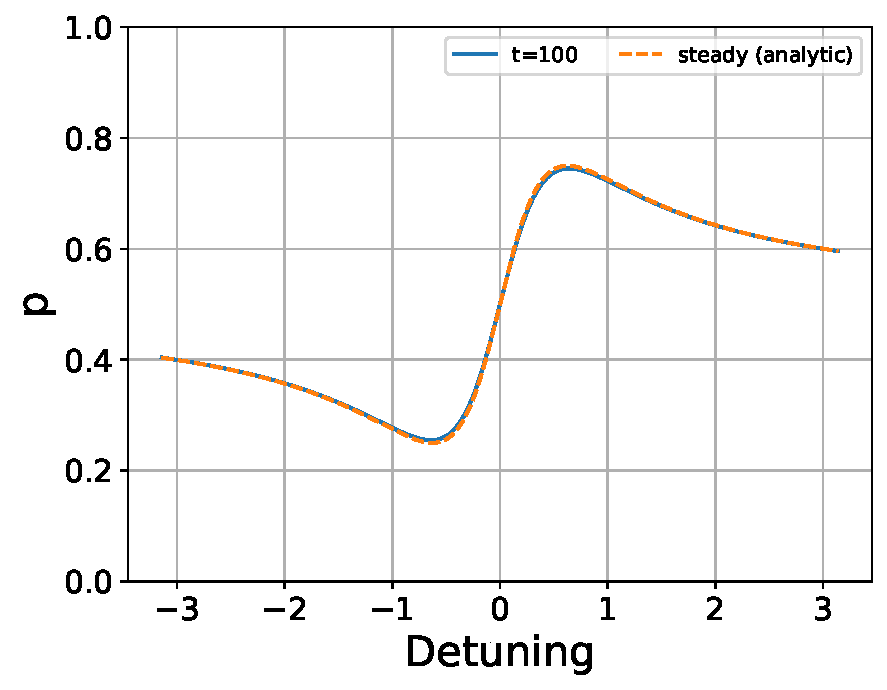
\includegraphics[width=8cm]{../../euriqa/calculations/master_equation/imgs/coherent-scatter_det_theory.pdf}
  \caption{Comparison between the analytic steady state population of $|1\rangle$
    and numerical result from master equation simulation.}
  \label{fig:compare-steady}
\end{figure}

We can compare this with the numerical simulation
result~(Fig.~\ref{fig:compare-steady}) showing very good agreement.

\end{document}
